\section{eval-extra}



\subsubsection{Simulator validation}
\label{sec:validation}

\begin{figure}[h]
\centering
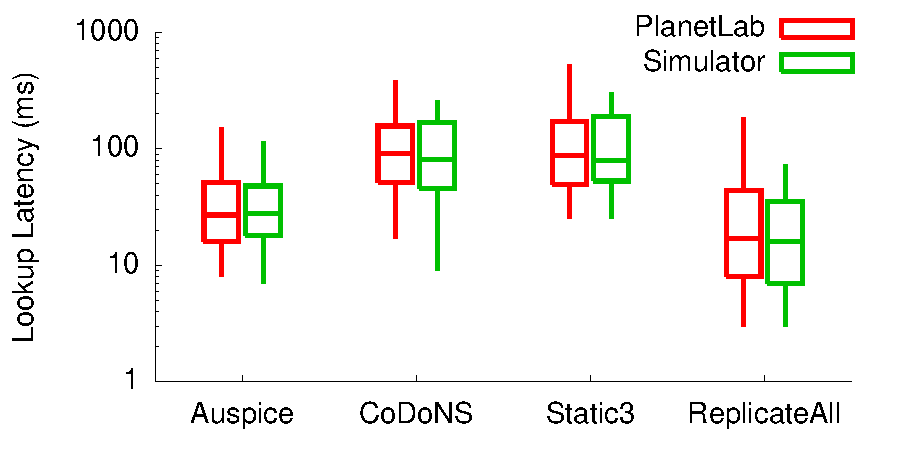
\includegraphics[scale=0.5]{graph/simulatorval1.pdf}
\vspace{-0.1in}
\caption{Latency across names on PlanetLab compared to simulator. Boxplot shows 5th, 25th, 50th, 75th and 95th percentile latencies.}
\vspace{-0.1in}
\label{fig:simulatorval}
\end{figure}

%\bp{How we do simulator validation}
We use a simulator for experiments in Section \ref{sec:optimal} and Section \ref{sec:sensitivity}.  To ensure the accuracy of the simulator, we first validate it based on an experiment on PlanetLab. 
In simulation,  server latency is calculated using  a queueing-theoretic model \cite{mm1} and network latency between two nodes is the measured RTT between corresponding PlanetLab nodes.  
We introduce a similar packet loss rate in the simulator as seen on PlanetLab. 
Figure \ref{fig:micro} shows a box plot of the distribution of median lookup latencies of names  in the PlanetLab experiment and in the simulator. We find that median latencies for all schemes in the simulator are within 8\% of that on PlanetLab. The 95\% latencies are higher on PlanetLab experiments than in simulator due to unpredictable wide-area latencies and server processing delays. 





\subsection{Analysis of \auspice\ design}
\label{sec:microbenchmark}

\begin{figure}[ht]
\centering
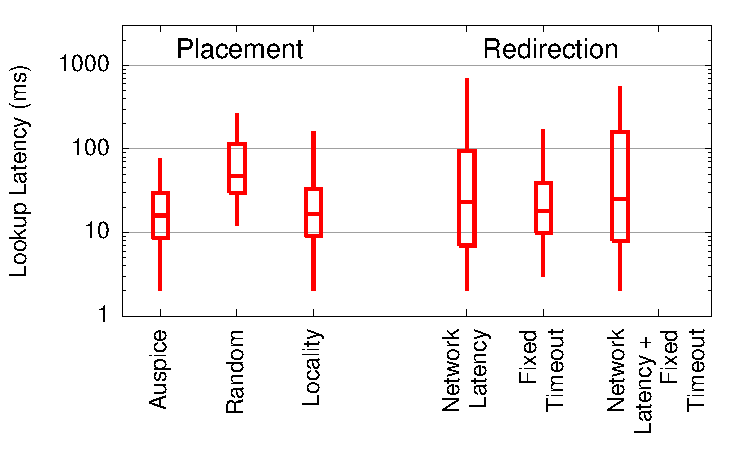
\includegraphics[scale=0.55]{graph/system-exp/mb-stats.pdf}
\vspace{-0.1in}
\caption{If \auspice\ uses a random placement, it has 4$\times$ higher median latency. If \auspice\ redirects  based on network latency, excluding server latency, it incurs a  3$\times$ higher 75 \%-ile latency.}
\vspace{-0.1in}
\label{fig:micro}
\end{figure}


%Our next experiment presents micro benchmarks for \auspice. 
%and shows that both its locality-aware placement and its load-aware redirection scheme help to achieve lower latencies. 
The aim of this experiment is to analyze which components of \auspice's design contribute most to its  performance.
We evaluate variants of \auspice's placement and redirection components, and group the results into two categories, placement and redirection, depending on which aspect of \auspice's design is varied. The experiment is conducted on PlanetLab with a similar workload as in Section \ref{sec:lowload}.
Figure \ref{fig:micro} shows the 5th, 25th, 50th, 75th, and 95th percentiles of the distribution of median lookup latencies of names for all variants of \auspice.

%The micro benchmarks performed on PlanetLab evaluate variants of \auspice's design, and we group our results into two categories, placement and redirection, depending on which aspect of \auspice's design is varied. Figure \ref{fig:micro}  presents results for all \auspice\ variants, and shows 5th, 25th, 50th, 75th, and 95th percentiles values of the distribution of median lookup latencies of names.

We evaluate two variants of \auspice's placement algorithm, \uniform\ and \locaware. 
These schemes choose the same number of replicas as \auspice, 
but \uniform\ chooses all replicas randomly to maximize load balance, 
and  \locaware\ chooses all replicas based on demand locations.  In Figure \ref{fig:micro},  \uniform\ has 4$\times$ higher median latencies than \auspice; \locaware\ and \auspice\ have nearly equal latencies until the 75th percentile.  
A locality-aware placement  (\auspice\ and \locaware) outperforms random placement because of geo-locality in the workload and because all schemes replicate 80\% of names at less than 15\% of nodes. Thus, we find that a locality-aware placement in \auspice\ is important to achieve good performance.

\eat{
Three alternative redirection strategies that we evaluate are: 
(1)  \textsf{Network-Latency}: Estimates latency to name server  only based on network latency, excluding server latency. 
(2)  \textsf{Fixed-Timeout}: Instead of using adaptive timeout, we use a fixed timeout of 150ms which is equal to 95th percentile lookup latency of \auspice\ in Figure \ref{fig:querylatencycdf}. 
(3) \textsf{Network-Latency + Fixed-Timeout}: Combination of (1) and (2).  Figure \ref{fig:micro} shows that  \textsf{Network-Latency}  has a 3$\times$ higher 75th percentile latency and a 9$\times$ higher 95th percentile latency compared to \auspice. This is because sever latency estimates  help identify PlanetLab nodes that are experiencing high load, and help in choosing lightly loaded name servers.  \textsf{Fixed-Timeout} performs comparable to \auspice\ until the 75th percentile, but has a 2.3$\times$ higher 95th percentile latency than an adaptive timeout. While it is possible to choose a fixed timeout value more carefully, adaptive timeout provides good performance without careful parameter tuning. This comparison shows that redirection based on combined network  \& server latency is a key factor in \auspice's performance. 
}

We evaluate three  alternative redirection strategies. 
(1)  \textsf{Network-Latency}:  Latency to name server is estimated  only based on network latency, excluding server latency. Figure \ref{fig:micro} shows that  \textsf{Network-Latency}  has a 3$\times$ higher 75th percentile latency and a 9$\times$ higher 95th percentile latency compared to \auspice. This is because server latency estimates  help identify PlanetLab nodes that are experiencing high load, which reduces request timeouts and improves latency. 
(2)  \textsf{Fixed-Timeout}: Instead of using adaptive timeout, we use a fixed timeout of 150ms which is equal to 95th percentile lookup latency of \auspice\ in the experiment in Section \ref{sec:lowload}. \textsf{Fixed-Timeout} performs comparable to \auspice\ until the 75th percentile, but has a 2.3$\times$ higher 95th percentile latency than an adaptive timeout. While it is possible to choose a fixed timeout value more carefully, adaptive timeout provides good performance without careful parameter tuning.
(3) \textsf{Network-Latency + Fixed-Timeout}: A combination of (1) and (2) which performs similar to \textsf{Network-Latency}. 
Overall, this comparison shows that redirection based on combined network  \& server latency is a key factor in \auspice's performance.



\eat{

\begin{figure*}[t]
\begin{minipage}[b]{0.3\linewidth}
\centering
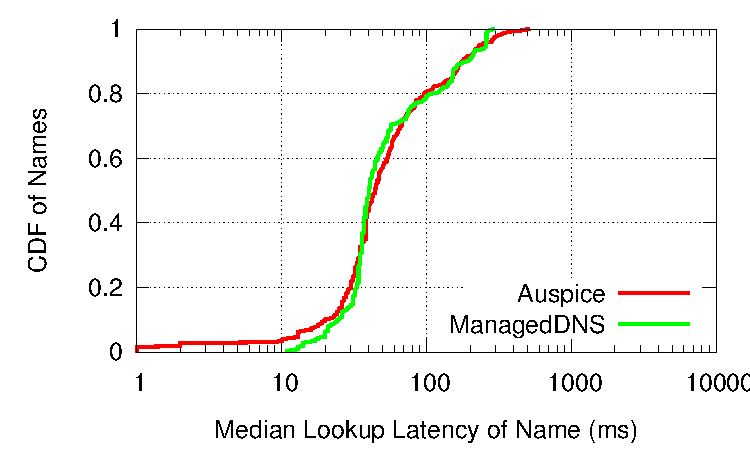
\includegraphics[scale=0.45]{graph/system-exp/dns-names.pdf}
\caption{\auspice\ has median latencies comparable  to managed DNS provider by placing only 5 resolvers in a locality-aware manner.}
\label{fig:manageddns}
\end{minipage}
\hspace{0.5cm}
\begin{minipage}[b]{0.3\linewidth}
\centering
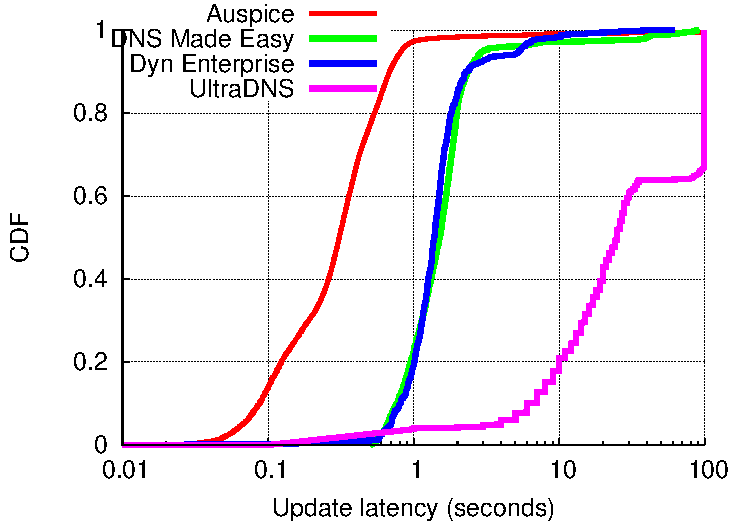
\includegraphics[scale=0.45]{graph/updatelatencycdf.pdf}
\caption{\auspice\ has an  update latency that is up to tens of seconds lower than managed DNS services.}
\label{fig:manageddnsupdate}
\end{minipage}
\hspace{0.5cm}
\begin{minipage}[b]{0.3\linewidth}
\centering
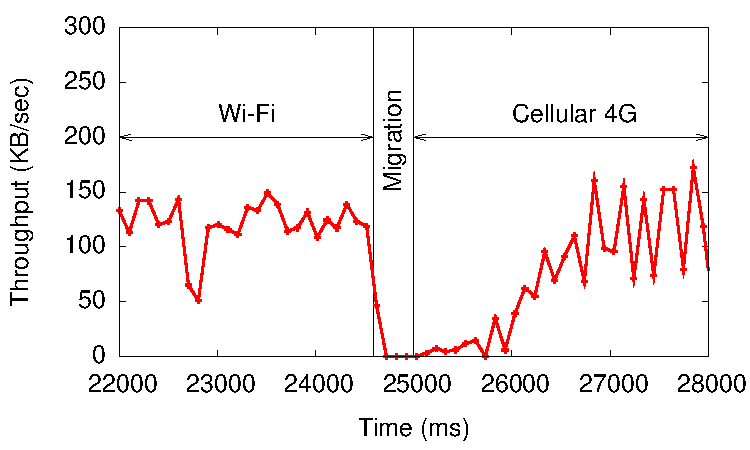
\includegraphics[scale=0.45]{graph/system-exp/Plot.pdf}
\caption{Connection migration from Wi-Fi to 4G. Migration starts at 24585 ms and ends at 24997 ms.}
\label{fig:mobility}
\end{minipage}
\vspace{-0.15in}
\end{figure*}

}

\subsection{Workload sensitivity analysis}
\label{sec:sensitivity}


This section presents sensitivity analysis of the following parameters in our synthetic workload for device names:  
%(1) ratio of service names to device names 
(1) geo-locality (2) ratio of  lookups to updates.
We perform these experiments with our simulator  as it enables us to explore a wider range of parameter values.  
Unless otherwise specified, all experiments in this section are performed with 10K name servers, 2K local name servers, 10K service names, and 100K device names. 
The latency metric we present is the median of the distribution of median lookup latencies of names.
%TBD: What is the ratio of lookups to updates for device names? What is the ratio of lookups for device names to lookups for service names?



%%Uncomment this after updating the figure 
\eat{
\begin{figure}
\centering
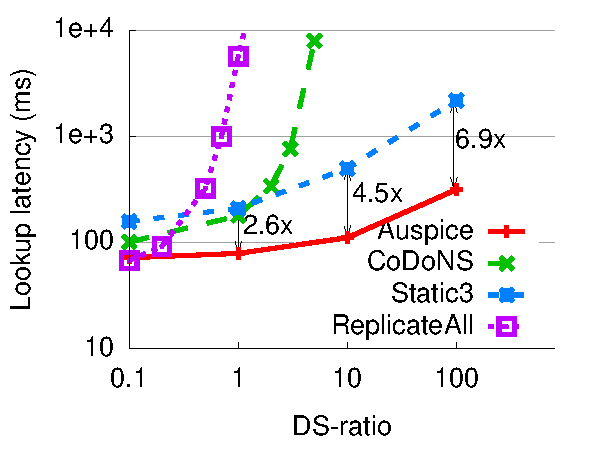
\includegraphics[scale=0.5]{graph/medianlatencyVSnummobile.pdf}
\vspace{-0.1in}
\caption{[Simulator] \auspice\ gives greater latency gains over \staticthree\ as the number of device names increases in  the workload.}
\label{fig:varymobile}
\end{figure}

\textbf{Ratio of device names to service names:} This experiment evaluates schemes for workloads with different ratios of device names to service names, called \emph{DS-ratio} for short.
We fix the number of service names to be 10K and vary the number of device names between 1000 to 1,000,000.
Figure \ref{fig:varymobile} presents our results.
\replicateall\  saturates server capacity for a workload with  DS-ratio = 1 due to high update costs. 
\auspice\  supports workloads with DS-ratio up to 100  as it minimizes the update cost for device names. 
Due to its locality-aware design, \auspice\ has  2.6$\times$, 4.5$\times$ and 6.9$\times$ lower latency than \staticthree\ when DS-ratios are 1, 10 and 100 respectively. 

\textcolor{blue}{
 \codons's latency increases more sharply than \auspice\ and \staticthree\  on increasing the number of device names.  
\codons\ creates  a greater number of replicas for device names than \auspice\ and \staticthree, which increases update cost and, as a result, the lookup latency for \codons.
For example, for a workload with DS-ratio = 2  and an average hop count of 2.0, \codons\ creates an average of 24 replicas/name compared to three replicas/name for \staticthree. We experimented with average hop-count values as high as 10, but the number of replicas did not reduce further.}
}
%, while using the recommended value of 16 for Pastry DHT's base parameter \cite{codons-paper}. 
%To reduce the number of replicas for \codons, we experimented with average hop count values up to 20 while using the recommended value of 16 for Pastry DHT's base parameter \cite{codons-paper}. But \codons\  still created more replicas  than \staticthree\ and \auspice.

% TBD: Figure 8 (DS-ratio) and Figure 9 (Geo-locality) are inconsistent. Our default DS-ratio is 10. In figure 8, Codons has higher latency than Static3 for DS-ratio = 10, but in figure 9 at Geo-locality of 1, Codons has lower latency than Static3 for  DS-ratio = 10.





\textbf{Geo-locality:}  In earlier experiments, 90\% requests for a device name show a strong geo-locality and 10\% requests originate from random  locations. 
We vary the workload geo-locality by changing the fraction of requests that originate from random  locations.  A \emph{geo-locality} of $p$ means (1-$p$) fraction of requests originate from random  locations.

Figure \ref{fig:varylocality} compares the latency for workloads with varying levels of geo-locality.
Both \staticthree\ and \codons\ are locality-unaware schemes, and therefore their latency remains the same irrespective of workload locality. But \auspice\ can achieve better latencies  as the geo-locality in the workload increases. Even in a workload with zero locality,   \auspice\ outperforms \staticthree\ by 2$\times$ because it creates more than three replicas for each name,  and outperforms \codons\ by $2.5\times$  because it redirects requests to the closest replica of a name, unlike \codons.

\begin{figure}
\centering
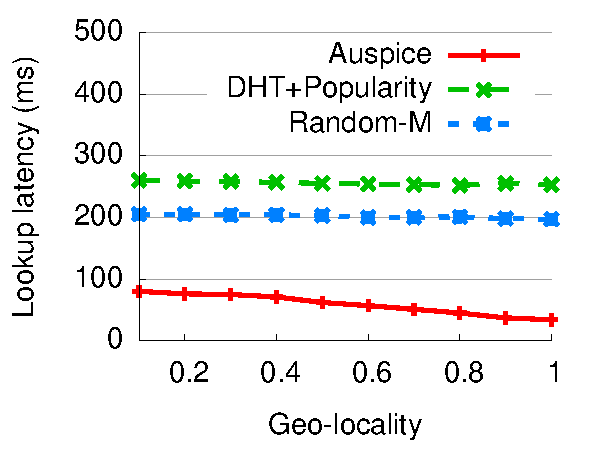
\includegraphics[scale=0.5]{graph/medianlatencyVSlocality.pdf}
\vspace{-0.1in}
\caption{[Simulator] \auspice\ outperforms other schemes by 2$\times$ to 5$\times$  across all locality levels. \replicateall\ has  100\% request failure rate  (not shown).}
\label{fig:varylocality}
\vspace{-0.1in}
\end{figure}

% TBD: limit all lines at 5 percent loss rate, at which they are assumed to reach capacity.


\textbf{Ratio of lookups to updates:} 
We vary the ratio of lookups to updates, termed as \emph{RW-ratio}, by increasing the number of lookups in the workload, but keeping the number of updates fixed. Figure \ref{fig:readwriteratio} shows that \auspice\ provides lower latencies for RW-ratios $>$ 1 as well as $<$ 1 instead of the default value of RW-ratio = 1 used in earlier experiments. As RW-ratios increase beyond 1,  \auspice\ handles the increase in number of lookups in the workload by decreasing the replication parameter $\beta$ (refer to \ref{eq:beta}). Lower $\beta$ values reduce number of replicas and hence the update costs for \auspice, which helps \auspice\ accommodate workloads with  RW-ratio $>$ 1. Reduced number of replicas increases  lookup latency of \auspice, but still \auspice\  has 2.95$\times$ lower latency than \staticthree\  for RW-ratio = 10. At RW-ratio > 5, \codons's latency is higher than both \staticthree\ and \auspice. This is because  \codons\ creates identical number and location of replicas for every name at all RW-ratios $>$ 1; tuning the hop-count parameter does not reduce the number of replicas further. Thus, \codons\ update cost remains the same, but increase in RW-ratio adds to the load-induced latency at name servers, which reflects in increased lookup latency for \codons.


\begin{figure}
\centering
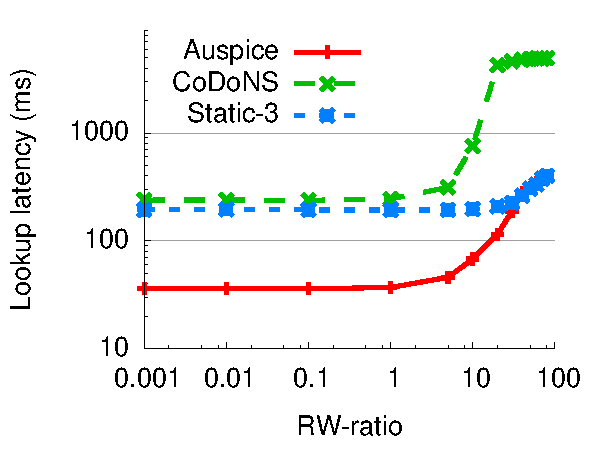
\includegraphics[scale=0.5]{graph/readwriteratio.pdf}
\vspace{-0.1in}
\caption{[Simulator] Ratio of lookups to updates for device names. For a lookup-dominated workload (RW-ratio = 10), \auspice\ has 2.95$\times$ lower latency than \staticthree.  \replicateall\ has 100\% request failure rate (not shown).}
\label{fig:readwriteratio}
\vspace{-0.1in}
\end{figure}



\subsection{TTL caching}

\textcolor{blue}{
We develop a simple analytical model to calculate the optimal TTL for a name at a cache that minimizes the connection-setup delay to the name. 
Using simulations of a TTL-based cache of name records, we show that the optimal TTL values predicted by our model are effective in miming connection-setup delay to names with a wide range of update to lookup ratios.}

%Using simulations of a TTL-based cache of name records, we show that the optimal TTL value to minimize the connection-setup delay  depends on the update to lookup  ratio of a name record. Further, we develop a simple analytical model to calculate the optimal TTL for a name at a cache. 


\textcolor{blue}{
In simulations, we consider a single name record and a single TTL-cache at a local name server. 
The update rate of the name is $w$,   the lookup rate of the name at the cache is $r$ and its TTL value at the cache is $t$. 
The inter-arrival times of updates and lookups are exponentially distributed.
At start, TTL cache is assumed to have fresh copy of the name. 
Thereafter, the cache entry can be in one of the three states:  (1)  State A: TTL has not expired and cache entry is fresh (2) State B: TTL has expired (3) State C: TTL has not expired and cache entry is stale due to an address update. For simplicity, we assume that cache evictions due to addition of other name records to the cache have a negligible probability.  }

%  The latency from user to the cache is much smaller than the latency to the other end-point of the connection, which is typical for Internet users.
%The connection setup time for a connection  starting from the time a user send a lookup request to the cache until connection setup is complete  depends on cache's current state. 
\textcolor{blue}{
The time to setup a connection to a name including the time to lookup the name record from the cache depends on the current state of the cache. 
The connection time is shortest for State A (cache hit) because name record lookup from the cache at local name name server  adds near zero overhead to the connection establishment time, which is typical for Internet users.
The connection time is slightly longer for State B (expired TTL) because the cache looks up the name record from an active replica in \auspice. 
The connection time is longest for State C because the cache returns an incorrect address to the user. The user first attempts to connect to the wrong address and after waiting for 2-3 round trip times, the connection setup times out. Next, user forces the cache to get the correct name record from \auspice\ and finally establishes the connection. 
The factor by which connection setup time increases due to a name lookup is taken to be $l_1 = 1$, $l_2 = 1.5$, and $l_3 = 4$ respectively for the above three cases. 
}

\textcolor{blue}{
We develop an analytical model to calculate the expected latency inflation factor for a name. To simplify  analysis, we assume that instead of a fixed TTL value $t$, TTL values  are drawn from an exponential distribution with mean $t$. The closed form expression for the expected latency inflation factor $L$ is as follows:
\label{eqn:expected_delay}
\[L =  l_1 \frac{r}{t+r+w} + l_2\frac{ t}{t+r} +  l_3 \frac{rw}{(t+r)(t+r+w)}\]
}
\textcolor{blue}{
\noindent
We use the above equation to calculate the TTL value which minimizes the expected delay, called \emph{Model-Opt-TTL}.  Figure \ref{fig:meanlatencyinflationfactor} shows the mean latency inflation factor (y-axis) for several values of ratios of TTL to update interval (x-axis) and update to lookup ratios (each line).  For each value of update to lookup ratio, we also show the Model-Opt-TTL and the corresponding  latency inflation factor. 
}

\textcolor{blue}{
We make two observations from Figure \ref{fig:meanlatencyinflationfactor}. 
First, the minimum value of the latency inflation factor reduces from 1.5  (= $l_2$) to 1.0 (= $l_1$) as the update to lookup ratio reduces. When updates are much more frequent than lookups, nearly all lookups require the cache to contact an active replica; hence, the minimum latency inflation is close to 1.5.
Conversely, when lookups are much more frequent than updates, suitably choosing a TTL value results in a high fraction of TTL-cache hits and hence minimum latency inflation is close to 1.0. 
Second,  Model-Opt-TTL gives a latency inflation factor  which is close the minimum latency inflation factor for each curve. Hence, our model helps select TTL-values that are effective is effective in reducing the latency inflation factor.
}

%This experiment evaluates how the TTL caching affects user-perceived latency and load on the name servers. TTL affects user-perceived latency in three ways: (a) when TTL hasn't expired and record is fresh, the client does nothing; (b) when the TTL has expired, the client contacts to the name server for a fresh record; (c) when the TTL hasn't expired but the record is stale because of mobility, the client  times out and then reconnects to the name server. We use a latency inflation factor to measure the above three scenarios and assign a factor of 1, 1.5 and 4 corresponding to them respectively. The writes are global and reads are distributed across 100 local name servers. Explain the process. times out from what? 

%Figure \ref{fig:medianlatencyinflationfactor} shows the median latency inflation factor we vary the TTL caching value. When write-to-read ratio is less than 1, the median inflation factor decreases as TTL increases. When write-to-read ratio is greater than 1, the median inflation factor increases as TTL increases. Figure \ref{fig:meanlatencyinflationfactor} shows the mean latency inflation factor. All lines first decrease and then increase, indicating that there is an optimal TTL value that results in the lowest latency.

%To derive the optimal TTL value, we make the following assumptions. Suppose the TTL is $T$, read rate $r$, and write rate $w$. After each refresh, the record is reused for min$(T,1/w)$ time. Thus, the fraction of reads that incur a non-zero latency is roughly $1/(r * \min(T,1/w))$. The fraction of requests that time out will be $(T * w) * (w/r)$ and the fraction of requests that result in a refresh because of TTL expiration will be $1/(r * T)$. 
%We further use $a$, $b$, $c$ to denote the latency inflation factor for requests that experience non-zero latency, timeouts and TTL expiration respectively, then when $T \leq 1/w$,  the optimal TTL value is $1/w * \sqrt{(a+b)/c}$; when $T \geq 1/w$, the optimal TTL value is $1/w * \sqrt{b/c}$.


%Figure \ref{fig:fractionrequest} shows the fraction of requests that are sent to the name servers because of TTL expiration or end-user mobility. As we expected, the fraction decreases as TTL increases, because longer TTL reduce the load incurred at the name servers. 


\begin{figure}[t]
\centering
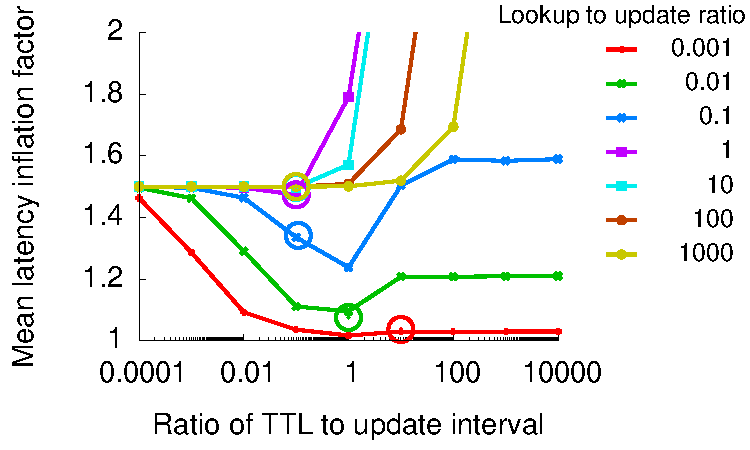
\includegraphics[scale=0.5]{graph/ttl.pdf}
\vspace{-0.1in}
\caption{[Simulator] Mean latency inflation factor as a function of TTL.}
\label{fig:meanlatencyinflationfactor}
\vspace{-0.1in}
\end{figure}

